\documentclass[a4paper]{article}


\usepackage[utf8]{inputenc}
\usepackage[german]{babel}
\usepackage{amsmath}
\usepackage{amssymb}
\usepackage{fancyhdr}
\usepackage{color}
\usepackage{graphicx}
\usepackage{lastpage}
\usepackage{listings} 
\usepackage{tikz}
\usepackage{pdflscape}
\usetikzlibrary{trees}
\usepackage{subfigure}
\usepackage{float}
\usepackage{polynom}
\usepackage{hyperref}
\usepackage{tabularx}
\usepackage{forloop}
\usepackage{geometry}
\usepackage{listings}
\usepackage[]{algorithm2e}
\usepackage{fancybox}
\usepackage{tikz}
\usetikzlibrary{shapes}

\usepackage{algorithmic}
\usetikzlibrary{automata,arrows}

\usepackage{xparse}
\input kvmacros

%Größe der Ränder setzen
\geometry{a4paper,left=3cm, right=3cm, top=3cm, bottom=3cm}

%Kopf- und Fußzeile
\pagestyle {fancy}
\fancyhead[L]{}
\fancyhead[C]{Artificial Intelligence}
\fancyhead[R]{\today}

\fancyfoot[L]{}
\fancyfoot[C]{}
\fancyfoot[R]{Seite \thepage /\pageref*{LastPage} }


%Formatierung der Überschrift, hier nichts ändern
\def\header#1#2{
\begin{center}
{\Large\bf Übungsblatt #1} %Blatt eintragen

{(Abgabetermin #2)}
\end{center}
}

%Definition der Punktetabelle, hier nichts ändern
\newcounter{punktelistectr}
\newcounter{punkte}
\newcommand{\punkteliste}[2]{%
  \setcounter{punkte}{#2}%
  \addtocounter{punkte}{-#1}%
  \stepcounter{punkte}%<-- also punkte = m-n+1 = Anzahl Spalten[1]
  \begin{center}%
  \begin{tabularx}{\linewidth}[]{@{}*{\thepunkte}{>{\centering\arraybackslash} X|}@{}>{\centering\arraybackslash}X}
      \forloop{punktelistectr}{#1}{\value{punktelistectr} < #2 } %
      {%
        \thepunktelistectr & 
      } 
      #2 &  $\Sigma$ \\
      \hline
      \forloop{punktelistectr}{#1}{\value{punktelistectr} < #2 } %
      {%
        &
      } &\\ 
      \forloop{punktelistectr}{#1}{\value{punktelistectr} < #2 } %
      {%
        &
      } &\\ 
    \end{tabularx}
  \end{center}
}



\begin{document}

%Hier bitte Student 1 usw ersetzen
\begin{tabularx}{\linewidth}{m{0.2 \linewidth}X}
\begin{minipage}{\linewidth}%
%
% ----------------------- TODO ---------------------------
%Hier Namen eintragen
%
Marc Tomasek \\
Marius Hobbhahn \\
\end{minipage} & \begin{minipage}{\linewidth}%
%
% ----------------------- TODO ---------------------------
%Die zweite Zahl durch die Anzahl der Aufgaben ersetzen
%
%
\punkteliste{1}{3} %
%
\end{minipage}\\
\end{tabularx}



% ----------------------- TODO ---------------------------
%
%Hier Nummer und Datum aktualisieren
\header{Nr. 6}{06.12.2017}
%---------------------------------------------------------------------------
\section*{Aufgabe 1} %Simulated Annealing
\subsection*{a} %Prinzip und Sinn
Simulated annealing is a hillclimbing variant which always allows 'uphill' moves, but also allows 'downhill' moves with a probability $p$, which is exponentially reduced with a decreasing 'temperature' $T$. It can sometimes find the global maximum where normal hillclimbing can't.

\subsection*{b} %Berechnung
\begin{table}[h]
	\centering
	\label{my-label}
	\begin{tabular}{|l|l|l|l|l|l|l|l|}
		\hline
		$n$ & $x_n$ & $\Delta x_n$ & $E(x_n)$ & $E(x_n + \Delta x_n)$ & $T_n$ & $P(x_n + \Delta x_n, x_n)$ & $r_n$ \\ \hline
		0   & 0.85  & -0.1         & 0.65     & 1.77                  & 1.6   & 1                          & 0.3   \\ \hline
		1   & 0.75  & -0.15        & 1.77     & 1.24                  & 0.8   & 0.52                       & 0.7   \\ \hline
		2   & 0.75  & -0.5         & 1.77     & 0.95                  & 0.4   & 0.13                       & 0.01  \\ \hline
		3   & 0.25  & 0.1          & 0.95     & 0.61                  & 0.2   & 0.19                       & 0.1   \\ \hline
		4   & 0.35  & 0.2          & 0.61     & 0.72                  & 0.1   & 1                          & 0.8   \\ \hline
		5   & 0.55  & 0.05         & 0.72     & 1.24                  & 0.05  & 1                          & 0.6   \\ \hline
	\end{tabular}
\end{table}


\subsection*{c} %Jemals Maximum
We are on the fifth step at the point $(0.55, 0.72)$.
\begin{center}
	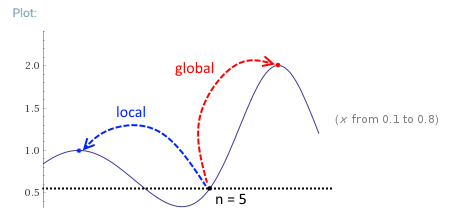
\includegraphics{a1c.png}
\end{center}
Because of $T_{n+1} = 0.5 \cdot T_n$, acceptance of values $E(x_{n+1}) < E(x_n)$ will become more and more rare, which leads to a low probabilty of moving away from the global maximum. \\
The chance of choosing values $E(x_{n+1}) > E(x_n)$ is uninfluenced and remains $1$, which likely leads to a steady ascent towards the global maximum at $(0.7, 2.0)$ if we get small step-sizes. \\
If in the unlikely event of a big negative step-size, for example $\Delta x_n = -0.3$ (where $E(x_{n+1}) > E(x_n)$), we could end up on the slopes of the local maximum at $(0.2, 1.0)$, which could lead to us not finding the global maximum, if no similar event occurs to get us back on the other slope (within our allowed runtime). \\\\
If our runtime is infinite, we will always find the slopes of the global maximum from the local maximum with a step-size $0.38 < \Delta x_n < 0.61$.\\
In conclusion, it is likely that we find the global maximum.






















\end{document}